\chapter{Referenzproblem und Datengrundlage}
Untersucht wird ein linear-elastischer Quaderbalken, der an einer Stirnfläche fest eingespannt und an der anderen durch eine gleichmäßig verteilte $z$-gerichtete Flächenlast beansprucht wird. Die Geometrie wird für jeden Fall neu vernetzt. Die FEM-Lösung wird auf ein gemeinsames normiertes Raster mit $21\times5\times5=525$ Punkten interpoliert. Ausgegeben werden die drei Verschiebungskomponenten in Metern. Für die Stützfläche wird im gemeinsamen Raster die bekannte homogene Verschiebungsrandbedingung gesetzt.

Die sechs Eingaben und ihre Trainingsgrenzen sind in Tabelle~\ref{tab:grenzen} angegeben. Der Trainingspool umfasst je 384 Fälle aus zwei Erzeugungsblöcken. Die Auswahlen sind blockausgeglichen und für die Größen 48, 96, 192, 384 und 768 verschachtelt. Drei Auswahlen dienen der Untersuchung kleinerer Trainingsmengen; bei 768 Fällen sind sie identisch. Für neuronale Vollpoolmodelle werden zusätzlich drei Initialisierungen betrachtet.
\begin{table}[htbp]\centering\caption{Parameter und Grenzen des Trainingsintervalls.}\label{tab:grenzen}
\begin{tabular}{llrr}\toprule Parameter & Einheit & Untergrenze & Obergrenze\\\midrule
Länge $L$ & m & 0,60 & 1,20\\ Breite $b$ & m & 0,06 & 0,10\\ Höhe $h$ & m & 0,08 & 0,14\\ Elastizitätsmodul $E$ & GPa & 70 & 210\\ Querkontraktionszahl $\nu$ & -- & 0,25 & 0,35\\ Kraft $F_z$ & N & $-1000$ & $-100$\\\bottomrule\end{tabular}\end{table}

Neben dem Trainingspool entstehen 128 neue Validierungs-, 256 Interpolations- und 128 Extrapolationsfälle. Validierungs- und Interpolationsparameter werden unabhängig innerhalb der Grenzen mittels Latin-Hypercube-Verfahren erzeugt. Ein Extrapolationsfall überschreitet genau eine Parametergrenze um 5--10\,\% der zugehörigen Intervallbreite. Die zwölf Parameter-/Seitengruppen enthalten je zehn oder elf Fälle. Parametervektoren werden gegen bekannte Designs und neue Kandidaten auf Überschneidungen in einer durch Intervallbreiten normierten Maximumsnorm mit Toleranz $10^{-10}$ geprüft.

Die FEM-Referenzen verwenden quadratische Elemente und den Netzdivisor 3. Fälle müssen physikalische und numerische Prüfungen einschließlich eines maximalen Auslenkungsverhältnisses von 0,02 erfüllen. Ein separater Pilot umfasst zwölf Extrapolationsfälle auf drei Netzstufen; er ist keine Garantie für Netzkonvergenz im gesamten Parameterraum. Euler--Bernoulli- und Timoshenko-Balkentheorie werden als Plausibilitätsreferenzen genutzt, nicht als exakte Lösungen aller Komponenten des dreidimensionalen Feldes.

\chapter{Methoden und Versuchsplanung}
\section{Konfigurationswahl und Datenrollen}
Die Modellauswahl erfolgt bei $N=384$ auf einer Trainingsauswahl und den 128 Validierungsfällen. Zielgröße ist der mittlere gewichtete relative Feldfehler. Bei Gleichstand folgen P95 und eine feste Konfigurationskennung; die zwei besten neuronalen Kandidaten werden mit drei Initialisierungen bestätigt. GPR wird nach einem deterministischen Protokoll abgestimmt. Für die Lernkurven bleibt danach je Familie dieselbe Konfiguration erhalten; eine separate Abstimmung je $N$ findet nicht statt. Abbildung~\ref{fig:ablauf} stellt die Trennung der Datenrollen dar.
\begin{figure}[htbp]\centering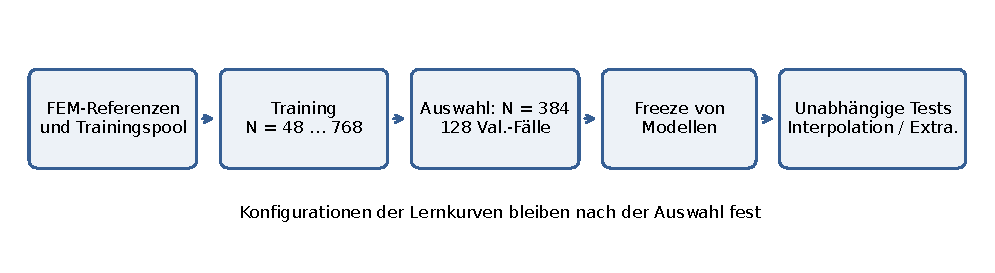
\includegraphics[width=\textwidth]{ablauf.pdf}\caption{Datenrollen und zeitliche Trennung der Modellwahl vom unabhängigen Test. Eigene Darstellung nach Studienprotokoll.}\label{fig:ablauf}\end{figure}

Die tatsächlich ausgewählten Einstellungen stehen in Tabelle~\ref{tab:config}. Die neuronalen Modelle verwenden Adam, höchstens 200 Epochen, eine Batchgröße von 32 und die Lernrate 0,001. GPR verwendet \texttt{ardmatern52}, einen linearen Mittelwert, ein konstantes numerisches Sigma von 0,001 und zwei Startlängenskalen. Die Quasi-Newton-Optimierung ist auf höchstens 500 Iterationen begrenzt. Der tatsächlich durchsuchte MLP-Raum umfasst Breiten 64 und 128, Tiefen 2 und 3, Lernraten 0,0005 und 0,001 sowie zwei Loss-Varianten; die ursprünglich vorgesehenen Breiten 32 und 80 fehlen.
\begin{table}[htbp]\centering\caption{Auf der Validierung ausgewählte Konfigurationen.}\label{tab:config}
\small\begin{tabular}{>{\raggedright\arraybackslash}p{25mm}>{\raggedright\arraybackslash}p{73mm}>{\raggedright\arraybackslash}p{30mm}r}\toprule Methode & Architektur beziehungsweise Kernel & Training / Loss & Rang\\\midrule
MLP & 3 Tanh-Schichten, Breite 128 & Adam, gew. Feld-MSE & --\\
RBF & 64 feste Gaußzentren, Breite 2; 2 Tanh-Schichten à 64 & Adam, gew. Feld-MSE & --\\
POD--MLP & 3 Tanh-Schichten, Breite 80 & Adam, gew. Feld-MSE & 2\\
POD--GPR & ARD-Matérn-5/2, linearer Mittelwert, Sigma 0,001 & exakte GPR & 15\\\bottomrule\end{tabular}\end{table}

\section{Kontrollierter POD- und Verteilungsvergleich}
Im kontrollierten POD-Vergleich werden die Ränge 2, 10 und 15 untersucht. POD--MLP und POD--GPR erhalten für denselben Rang, dieselbe Trainingsauswahl und Reihenfolge exakt denselben Mittelwert und dieselbe gewichtete Basis. Die Regressoreinstellungen der ausgewählten Familienkonfigurationen bleiben ansonsten fest. Die eigenständige Fit-Zeit wird als Summe aus der gemessenen Fit-Zeit mit vorbereiteter Basis und der separat gemessenen gemeinsamen POD-Zeit geschätzt.

Eine separate Untersuchung bei $N=192$ vergleicht eine raumfüllende mit einer auf niedrige Längen konzentrierten Auswahl. Beide sind blockausgeglichen und besitzen identische äußere Parametergrenzen. Die Bewertung erfolgt auf denselben unabhängigen Fällen.

\section{Freeze, Messung und Auswertung}
Vor Testlabelzugriff werden Konfigurationen, Daten- und Quellprüfsummen sowie die vorgesehenen Modellartefakte eingefroren. Die Tests werden anschließend getrennt nach Interpolation und Extrapolation ausgewertet. Die ursprüngliche Testauswertung brach nach dem ersten Modell wegen einer überschriebenen Manifestvariablen ab. Eine separat dokumentierte und gehashte technische Korrektur entstand nach dem ersten Testzugriff; Modelle, Auswahlregel und Metriken blieben unverändert. Für die beiden bereits berechneten Splits stimmen zwölf geprüfte numerische Fehler- und Referenzgrößen mit der Wiederholung überein. Die Korrektur ist somit dokumentiert, jedoch nicht nachträglich Teil des ursprünglichen Freeze.

Fit, Vorverarbeitung, POD beziehungsweise Zentrenaufbau, Regression, Suche sowie Laden und Speichern werden getrennt erfasst. Für vollständige Vorhersagen werden nach Warm-up wiederholte Einzelfall- und 128er-Batch-Aufrufe gemessen. Im Vollpool sind die drei neuronalen Wiederholungen unterschiedliche Netzinitialisierungen; zusätzliche deterministische GPR-Fits dienen ausschließlich der Zeitmessung.

Ein zusätzlicher, nachträglich angelegter Benchmark wählt vor der Messung zwölf Interpolationsfälle anhand fester Datenpositionen, unabhängig vom Vorhersagefehler. Auf derselben Maschine werden FEM-Lösung mit Feldinterpolation und vollständige Vorhersagen der eingefrorenen Modelle gemessen. Details und Kostenabgrenzung folgen in Kapitel~\ref{chap:ergebnisse}.
